\documentclass[11pt,a4paper]{article}
\usepackage[T1]{fontenc}
\usepackage[utf8]{inputenc}
\usepackage{lmodern}
\usepackage[margin=22mm]{geometry}
\usepackage{amsmath,amssymb,amsthm,booktabs,tabularx,array,longtable}
\usepackage{enumitem,xcolor,xurl,hyperref,etoolbox}
\usepackage{tikz}
\usetikzlibrary{arrows.meta,positioning}
\hypersetup{colorlinks=true,linkcolor=blue!55!black,urlcolor=blue!55!black,
  citecolor=blue!55!black,pdftitle={Native Inference: From Grounded Judgments to Composable Proof and Checking}}
\setlength{\emergencystretch}{3em}
\setlength{\parskip}{4pt}
\setlength{\parindent}{0pt}
\setlist{nosep,leftmargin=*}
\definecolor{ink}{HTML}{18344D}
\newcommand{\code}[1]{\texttt{\detokenize{#1}}}
\newcommand{\name}[1]{\textup{\Urlmuskip=0mu\relax\nolinkurl{#1}}}
\newcommand{\leanone}[1]{\leansep\name{#1}\gdef\leansep{, }}
\newcommand{\lean}[1]{\par\smallskip{\small\raggedright\sloppy\textbf{Lean.} \gdef\leansep{}\forcsvlist{\leanone}{#1}\par}}
\newcommand{\status}[1]{\par{\small\textbf{Status.} #1\par}}
\theoremstyle{plain}
\newtheorem{theorem}{Theorem}[section]
\newtheorem{proposition}[theorem]{Proposition}
\newtheorem{corollary}[theorem]{Corollary}
\theoremstyle{definition}
\newtheorem{definition}[theorem]{Definition}
\newtheorem{example}[theorem]{Example}
\theoremstyle{remark}
\newtheorem{remark}[theorem]{Remark}
\newcommand{\Term}{\mathsf{Term}}
\newcommand{\Free}{\mathsf{Free}}
\newcommand{\subst}{\mathsf{subst}}
\newcommand{\size}{\mathsf{size}}
\newcommand{\occ}{\mathsf{occ}}

\title{\color{ink}Native Inference\\[3pt]
  \large From grounded judgments to composable proof, computation and meaning}
\author{Mettapedia Working Notes}
\date{17 October 2026}

\begin{document}
\maketitle

\begin{abstract}
What must a reasoner supply for another reasoner to check an inference? We
begin with observations, explicitly admitted assumptions and licensed rule
instances. The formal foundation is an effective finitary presentation of
judgments, with contexts and binding kept explicit. The open derivations over
such a presentation form the free cartesian
multicategory on its rule instances; certificate trees are its closed
morphisms and shared derivation graphs unfold into them. Translations between
kernels are multifunctors, determined by the images of rule instances. Logical
work is additive under composition; contraction in a rule image separates tree
from graph representations, while extension by definitions changes the
multicategory itself. Atomic multi-pattern steps without consumption are graph
replay and are independent of the order of independent steps; a consuming
split/join process exceeds tree-shaped single-wire-cut composition. A finite
evidence checker connects circular strong Kleene specifications to the same
proof interface while distinguishing ungroundedness from unfinished checking.
Buddhist epistemology and the physical, qualitative, totality and indexical
distinctions of scrutability theory motivate explicit evidence boundaries;
these philosophical interpretations are distinguished from formal claims. The
ledger in Section~\ref{sec:ledger} records names, axioms and status, and
Section~\ref{sec:open} lists what is open.
\end{abstract}

\tableofcontents

\section{What makes a step of reasoning?}\label{sec:intuition}

A person sees smoke above a hill and concludes that there is fire. A program
matches a stored equation against a subterm and replaces it. A proof assistant
applies a lemma to two earlier results. These activities differ in their
objects, their sources of authority and their treatment of resources, but
they share a question: \emph{what licenses this conclusion from these particular
inputs, here?}

Consider the small mathematical inference
\[
 \frac{e_A : A \qquad e_{A\Rightarrow B} : A\Rightarrow B}
      {\mathsf{apply}(e_{A\Rightarrow B},e_A) : B}.
\]
The labels $e_A$ and $e_{A\Rightarrow B}$ record evidence, rather than an
unexplained assertion that $A$ and $A\Rightarrow B$ are true. Either input may
be an assumption, in which case the conclusion remains conditional on it.
Alternatively it may have a checked derivation. Recording the dependencies
lets another reader distinguish these cases. Modus ponens is one possible
licensed rule; it is not built into every rewrite language or every model of
reasoning considered here.

The corresponding rewrite example is
\[
  (\mathsf{add}\;\mathsf{Z}\;n)\longrightarrow n,
  \qquad
  \mathsf{S}(\mathsf{add}\;\mathsf{Z}\;\mathsf{Z})
        \longrightarrow\mathsf{S}(\mathsf{Z}).
\]
A fully specified recipe cites the admitted rule, the inner site, the
substitution $n:=\mathsf{Z}$ and any required side evidence. The checker
replays those choices. The rule does not automatically apply under every
constructor: the selected language must license the surrounding context.
An equality judgment, a directed execution step and a claim about an evaluator's
complete result multiset are different conclusions.

This is a foundation for checking licensed inferences, not a claim that all
reasoning is deduction. Induction, abduction, analogy and proof search suggest
claims or revise assumptions. Their own presentations may license probabilistic
updates or defeasible conclusions rather than truth-preserving deduction.
A checked Bayesian update, for example, certifies the stated calculation under
its model and observations; a high resulting probability is not a deductive
proof of the event. The common floor asks for the contract of each step.

\subsection{Observations, assumptions and checked consequences}

An observation enters a formal account through an interface: a sensor report,
a human assertion, a database snapshot, or a chosen mathematical model.
Checking a consequence of that report does not check that the sensor was
accurate. A certificate can establish
\[
  \Gamma,\mathsf{Report}(i,o)\vdash C
\]
while leaving the reliability and interpretation of the report as explicit
premises. This is useful even when a premise is defeasible: changing it
identifies which retained conclusions need revalidation.

We therefore separate three obligations. \emph{Admission} states which
assumptions, observations and declarations are available. \emph{Inference
checking} validates a finite composition under those admissions.
\emph{Semantic soundness} relates the admitted rules and their consequences to
a stated interpretation. None of these obligations is discharged by merely
printing a theorem-shaped atom. A sealed theorem value can enforce the
construction discipline inside an implementation; an exported certificate
permits independent replay. Their logical comparison is separate from the
runtime's unforgeability and lifetime guarantees.

\subsection{A dialogue with Buddhist epistemology}\label{sec:buddhist}

The school of Dignaga and Dharmakirti distinguishes perception from inference,
and inference for oneself from the presentation of an inference to another.
Dharmakirti's \emph{Nyayabindu} develops inferential knowledge through a reason
whose relevant characteristics must be established\cite{Nyayabindu}.
The familiar smoke/fire example makes the distinction practical: recognizing
smoke at this hill and licensing the connection to fire are different tasks.
A formal derivation records the connection and the cited instance; it cannot
manufacture reliable perception from the appearance of a valid derivation.

This motivates a division between finding a reason and presenting a checkable
reason. The connection to certificate checking is architectural, not an
identity between Buddhist epistemology and a modern proof calculus.
In particular, inference as valid cognition includes epistemic demands that
the replay of a formal certificate does not settle. The companion
\emph{Formal Buddhist Logic} studies precise readings of valid reasons,
non-perception, exclusion and four-corner evidence separately.

One consequence matters immediately: failure to observe is not, by itself,
evidence of absence. A negative conclusion requires a premise such as adequate
coverage, observability or an exhaustive finite check. Similarly, failure to
find a proof is not a proof of negation. Four-corner evidence, where positive
and negative support can both occur or both be absent, is useful for some
knowledge stores. It is not automatically the logic of every native kernel,
and neither four-corner evidence nor strong Kleene partial truth is simply
identified with the Buddhist fourfold analysis.

\subsection{Phenomenal and indexical grounding}\label{sec:pqti}

Chalmers's scrutability programme distinguishes physical information $P$,
phenomenal information $Q$, totality information $T$ and indexical information
$I$\cite{ChalmersJackson,ChalmersWorld}. Indexical information supplies a
location within an account; the totality component addresses what the account
excludes. These distinctions help ask what a formal reasoning system has been
given, but the scrutability thesis does not provide an executable kernel.

Our use is deliberately open-ended. Let $i:I$ specify an agent, stage or
location; let $p:P(i)$ specify publicly represented conditions; and let
$Q(i,p)$ record further qualitative distinctions. The indexed total space
\[
     \mathcal E=\sum_{i:I}\sum_{p:P(i)}Q(i,p)
\]
keeps the coordinates distinct. It does not assert that these families exhaust
possible experience or that qualitative information is recovered from public
data. Replacing the physical vocabulary by abstract laws $A$ gives an
$A/Q/I$ variant of this descriptive scheme; it is not a renamed assertion of
Chalmers's full $P/Q/T/I$ thesis. A local coverage certificate may authorize a
particular negative conclusion without committing to a global ``that's all''
claim about the world.

The immediate grounding for a human reasoner may include phenomenal
experience. A machine account instead requires a specified observation
interface; this paper does not establish that the interface is conscious or
that recording an experience report captures the experience itself.
The operational, intensional and extensional faces of inference are another
distinction: an execution, its retained proof evidence and its interpretation.
Their comparison maps are mathematical obligations. The three faces are not
identified term for term with $P$, $Q$ and $I$; in particular a proof's meaning
in a Henkin model is not thereby a phenomenal state.

\subsection{From a local step to a proof category}

A rule has typed input slots and a typed output. Filling its slots with
derivations constructs a larger derivation. Filling slots in stages or all at
once agrees by associativity; a premise hole is an identity. Multiple input
slots lead to a multicategory. A unary rewrite sequence gives the path-category
case. This is the elementary categorical content of proof composition, rather
than a demand that every language be encoded in one privileged logic.

\begin{center}
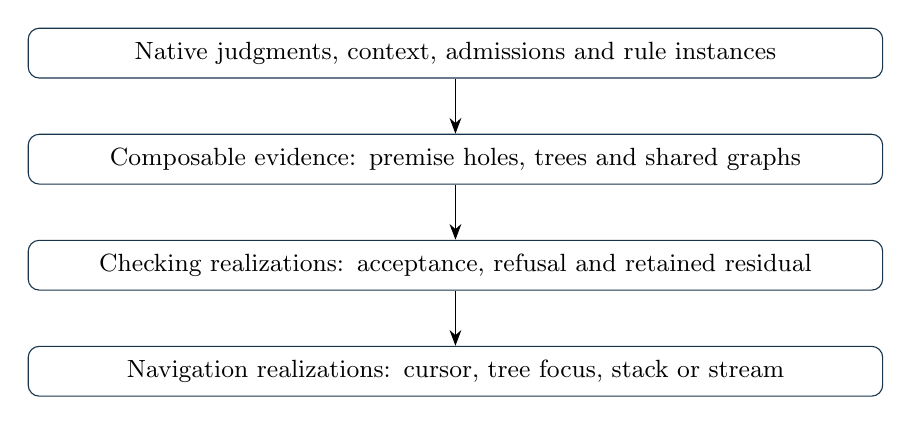
\begin{tikzpicture}[box/.style={draw=ink,rounded corners,align=center,
  text width=105mm,inner sep=5pt,font=\small},node distance=7mm,
  >={Stealth[length=2mm]}]
\node[box] (rules) {Native judgments, context, admissions and rule instances};
\node[box,below=of rules] (proofs) {Composable evidence: premise holes, trees and shared graphs};
\node[box,below=of proofs] (machine) {Checking realizations: acceptance, refusal and retained residual};
\node[box,below=of machine] (storage) {Navigation realizations: cursor, tree focus, stack or stream};
\draw[->] (rules) -- (proofs);
\draw[->] (proofs) -- (machine);
\draw[->] (machine) -- (storage);
\end{tikzpicture}
\end{center}

These are dependency levels, not successive authorities. A cursor's current
focus can be made observable, like a reader's position in a proof, but a
source calculus need not contain that position. Conversely a language that
makes scheduling or resource ownership observable needs a realization theorem
preserving precisely those observations. The model should follow those
semantics rather than the convenience of a particular storage backend.

\section{Scope and relation to the abstract-machine notes}\label{sec:scope}

The companion notes \emph{Abstract Machines} (Section~13, ``Proof machines:
scoped, licensed composition'') describe how source judgments, composable
evidence, checking realizations and navigation adapters are layered, and which
checking machines realize which kernels. This note does not repeat that
material. It supplies the mathematical structure of the evidence layer: what
composition of derivations is, how translations act on it, what costs are
attached to it, and how atomic multi-premise execution relates to it.

Section map.
\begin{center}\small
\begin{tabularx}{\linewidth}{lX}
\toprule
Section & Content \\
\midrule
\ref{sec:grounding} & Circular specifications, finite evidence and semantic partiality \\
\ref{sec:ladder} & The checking ladder and its distinct comparison axes \\
\ref{sec:free} & Rule signatures, open derivations and freeness \\
\ref{sec:kernels} & Kernels as free multicategories: trees, graphs and authored calculi \\
\ref{sec:translations} & Translations as multifunctors \\
\ref{sec:costs} & Costs: logical work, sharing (SHARE) and extension (EXTEND) \\
\ref{sec:execution} & Atomic multi-pattern steps and schedules \\
\ref{sec:revalidation} & Admission and revalidation of retained evidence \\
\ref{sec:modules} & Module coverage and the LRAT action adapter \\
\ref{sec:headline} & The costed HOL Light to MM0 translation \\
\ref{sec:ledger} & Status ledger \\
\ref{sec:open} & Open problems \\
\bottomrule
\end{tabularx}
\end{center}

\section{Circular specifications and finite evidence}\label{sec:grounding}

Circular syntax and circular justification are different. A finite collection
of named propositions can contain a reference cycle, while a particular
justification for one of its conclusions is still a finite, well-founded
tree. For example, if a grounded fact $G$ is true, then $L\lor G$ is true in
strong Kleene semantics even when $L$ refers negatively to itself. The
evidence uses $G$; it does not need a proof of $L$.

Let each judgment $j:J$ have a specification $\mathsf{spec}(j)$ built from base
facts, truth references, negation, conjunction and disjunction. A valuation
is a pair $(H,F)$ of positive and negative extensions, ordered by inclusion
in both coordinates. Strong Kleene evaluation induces a monotone jump
$\Phi(H,F)$. Starting with $(\varnothing,\varnothing)$ selects its least fixed
point $(H_*,F_*)$\cite{KripkeTruth}. With consistent base facts the two
extensions are disjoint. They need not cover $J$.

The liar $L=\neg\mathsf{truth}(L)$ receives neither polarity. The truth-teller
$U=\mathsf{truth}(U)$ also receives neither in the least fixed point, although
other fixed points can make it true or false. Merely checking that an offered
valuation is a fixed point therefore does not establish groundedness.

\begin{theorem}[Grounded evidence as a native proof profile]
For the existing strong Kleene specification system with decidable base
admission and decidable equality of judgment and base labels, ten local rule
codes give an exact rule-witness interface. A
judgment $j$ has a positive or negative grounded verdict exactly when there
exists an accepted finite certificate for its specification at that polarity.
Equivalently, that signed specification has a closed proof in the free
multicategory of the interface. These statements do not require $J$ finite.
\end{theorem}
\lean{KripkeTruth.Checking.interface, Checking.check_sound, Checking.coverage, Checking.judgment_coverage, Checking.closed_proof_iff_grounded}

The local rules are the source evidence constructors: admitted positive and
negative base leaves; explicit unfolding at a truth reference; polarity reversal
at negation; two positive premises for conjunction and either negative premise
to refute it; either positive premise for disjunction and two negative premises
to refute it. There is no rule that establishes a judgment merely by citing its
own label. Generic tree and graph checking apply without a new account of
proof composition. This is one particular partial-truth logic hosted by the
framework, not a change of every kernel to a three-valued object logic.

\begin{theorem}[Finite decision agrees with the certificate authority]
Under these assumptions, if $J$ is finite, iteration from the empty valuation reaches $(H_*,F_*)$ after
at most $2|J|$ jumps. The implemented Boolean-pair iteration returns a polarity
exactly when some finite certificate for that polarity is accepted.
\end{theorem}
\lean{KripkeTruth.System.stage_eq_least, System.groundedDecide_spec, Checking.finite_decision_iff_certificate}

The bound counts semantic jumps. It neither makes a jump constant time nor
proves that the current recursive evaluator avoids repeated work. It depends
on a finite judgment domain and decidable base admission. It is not a bound for
an unrestricted self-referential truth language with quantifiers.

\begin{example}[Completion is not bivalence]
The finite example computes the twice-ascribed fact as positive, a conjunction
with a grounded false component as negative, and the liar and truth-teller as
undetermined. The completed liar computation is not unfinished work. Conversely
the initially unknown fact becomes true at a later stage, so an intermediate
unknown value does not establish ungroundedness. The fact certificate with a
forged negative claim is refused, and a self-reference with no supplied premise
is refused. The liar has no finite certificate for either polarity.
\end{example}
\lean{KripkeTruth.Example.decided_verdicts, Checking.Controls.fact_accepts, Checking.Controls.forged_false_refuses, Checking.Controls.absent_premise_refuses, Checking.Controls.false_base_leaf_refuses, Checking.Controls.cyclic_graph_refuses, Checking.Controls.liar_has_no_certificate}

\subsection{Several meanings of an absent answer}

\begin{center}\small
\begin{tabularx}{\linewidth}{@{}>{\raggedright\arraybackslash}p{0.26\linewidth}X@{}}
\toprule
Outcome & What has been established \\
\midrule
Accepted certificate & This evidence checks for this claim under these admissions. \\
Refused certificate & This candidate fails checking; another candidate may prove the claim. \\
Negative evidence & A stated negative judgment, or an obstruction under the selected authority. \\
Grounded undetermined & Neither polarity belongs to the selected least fixed point. \\
Unfinished check & A retained residual remains; no final verdict follows. \\
Outside an effective profile & The selected checking method has no authority for this request. \\
Conflicting reports & A knowledge store has both supports; the chosen logic must specify their consequence. \\
\bottomrule
\end{tabularx}
\end{center}

The shared authority algebra already distinguishes evidence, obstruction,
fragment boundaries and restartable resource frontiers. The partial-truth
profile gives one mathematically stable meaning to a boundary. It must not
turn a timeout, a missing proof or an untrusted report into a falsehood.
Nor should the three-valued semantic result replace the richer execution
status. Both coordinates can be retained.
\lean{KripkeTruth.Checking.finite_undetermined_iff_no_certificates}

\subsection{Reflection, observation and open-endedness}

Self-reference imposes a precise local obstruction: when the liar equation is
required, no total Boolean fixed-point valuation satisfies the system. This
is not a theorem that every language containing a truth symbol is inconsistent.
Gödel incompleteness is a different obstruction: an appropriate consistent,
effective arithmetical theory cannot capture every truth of its intended
standard model. Reflection levels record which theory a claim concerns;
they do not grant an unqualified rule asserting the current theory's own
soundness. The existing consistency-tower results are parameterized by their
arithmetical hypotheses, which must be instantiated before a concrete base
theory is claimed.

Model observations have their own limitations. Indistinguishability by the
selected formulas is weaker than isomorphism; downward Lowenheim--Skolem
requires the relevant language and parameter cardinal bounds. First-order
theories can be categorical at a specified infinite cardinal, so the
finite-model observation cannot be generalized to prohibit such categoricity.
These model-theoretic qualifications do not alter the local rule checker.

Neither hypersets nor a terminal coalgebra are required for the evidence
profile above. A final coalgebra is final for a specified functor in a
specified category, not an automatic universe containing every possible
logic. Likewise, observer-relative indistinguishability does not justify
substitution in arbitrary contexts: a replacement theorem must establish the
congruence or naturality law for the contexts actually permitted.

\section{The checking ladder}\label{sec:ladder}

Tier zero names a checking discipline: supply finite evidence for licensed
rule applications, with explicit dependencies and enough local choices for a
terminating checker. It does not name a weakest axiom system, a unique primitive
basis, a universal notion of truth, or a promise of polynomial checking for
every possible encoding. A powerful set theory and a modest rewrite calculus
can both have this discipline.

\begin{center}\small
\begin{tabularx}{\linewidth}{@{}>{\raggedright\arraybackslash}p{0.25\linewidth}>{\raggedright\arraybackslash}X>{\raggedright\arraybackslash}X@{}}
\toprule
Presentation & Supplied evidence & Principal checking obligation \\
\midrule
Explicit rule replay & Rule instances, premises, substitutions and side witnesses & Replay each licensed composition. \\
Retained sharing & A dependency graph and selected root & Validate references and local instances without unfolding shared premises. \\
Compressed computation & A strategy, fuel and optional checkpoints & Reproduce the specified computation and its endpoint. \\
Theory extension & Declarations, definitions and admission evidence & State conservativity or new assumptions and revalidate reuse. \\
Reconstruction & Untrusted tactic or prover output & Produce a certificate that the destination independently checks. \\
\bottomrule
\end{tabularx}
\end{center}

This is a family of comparisons rather than one total ordering. Logical
strength, source expressiveness, certificate size, checking time, search power
and trusted implementation are separate axes. A proof-size translation does
not by itself prove a runtime bound. A faithful map on existing proofs need
not reflect the existence of proofs in its target. The intuitionistic-to-classical
inclusion below is a concrete example.

Fuel illustrates both the benefit and the price of compression. If a specified
machine accepts after $n$ reduction steps, supplying $n$ makes bounded replay
decidable and reproduces that successful run. A binary count needs only
logarithmically many bits, but replay can still take $n$ steps. Checkpoints
need justification between them; an explicit trace writes more information.
A trace's linear number of local checks is not automatically linear bit-time
if those local checks manipulate large substitutions or expressions.

The library already formalizes fuelled conversion evidence, explicit equality
recipes and reproducible strategy hints. It also keeps the Lean4Lean
algorithmic checker separate from ideal typing and conversion. More fuel
recovers a successful finite run; it cannot make an incomplete algorithm
complete for a larger ideal relation. The present executable Lean-related
instance is a specified head-conversion profile, not a proof that the full
Lean kernel has been reconstructed. The Lean4Less boundary records this
distinction rather than treating implementation heartbeats as portable
reduction counts.

The comparison target matters more than the implementation language. McTT
proves soundness and completeness of an extracted checker for its specified
Martin-Lof type theory\cite{McTT}. The observational theory $\mathsf{TT}_{obs}$
has a normalizing reduction and decidable conversion and type checking for its
own rules\cite{TTobs}. These are useful reference profiles; neither result is
a completeness theorem for Lean's different judgment, nor does implementing a
checker in Rocq identify its object theory with Rocq's full calculus. Runtime
efficiency requires a separate measurement.

\subsection{Weighted answers, effects and paid work}

A useful companion model of an effectful computation is
\[
 \mathsf{Spec}(K,C,W,X)
   = W\longrightarrow\mathsf{Ans}_K(X\times W\times C),
 \qquad \mathsf{Ans}_K(Y)=Y\to_{\mathrm{fin}}K.
\]
Here $K$ is a commutative semiring of answer annotations, $C$ a commutative
monoid of branch costs, and $W$ a world or space. Sequencing combines weights,
threads each branch's state and accumulates its cost. This supplies one lawful
model, not a complete semantics of every language that returns several answers.
Reads and writes need not commute. A weight is not automatically a probability,
a degree of truth or an unresolved scheduler choice. In particular the existing
no-distributive-law result concerns probability distributions over finite sets
with specified naturality and unit laws; it is not a prohibition on every
combination of probabilistic and nondeterministic operations.
\lean{LayerEffects.Spec.bind_assoc, LayerEffects.Controls.put_get_not_comm, NondeterminismProbability.no_distributiveLaw}

Two proved information-loss boundaries matter for inference. Charging a branch
and then failing leaves no successful answer carrying that charge; the total
paid work cannot in general be recovered from the surviving answers. It needs
an execution account with its own observation contract. Likewise marginal
positive/negative counts for $A$ and $B$ do not determine counts for $A\land B$
on the same worlds. Cartesian pairing of sample bags has a lawful product,
but that product does not recover unknown dependence. A proof checker can
validate either stated calculation without silently equating their meanings.
\lean{LayerEffects.Spec.no_failed_cost_recovery, EvidenceSpaces.no_same_world_conjunction_from_marginals}

These models belong downstream of the rule and evidence layer. A categorical
completion such as $\operatorname{Ind}(\mathcal C)$, or a dependent type theory,
requires its own objects, judgments and comparison theorems; neither follows
from the displayed computation type alone. Similarly, a checked absence
frontier proves a negative claim relative to its licensed future relation.
Identifying that claim with a guest logic's internal negation requires a
separate interpretation theorem.

\subsection{Three faces across the ladder}

The operational, retained-proof and semantic faces persist across the ladder.
An execution explains how checking proceeded, a proof records what licensed
the claim, and a semantic map explains what the claim means. A compiler or
optimization must name which face it preserves, which it reflects and what
information its observation forgets.

\begin{center}
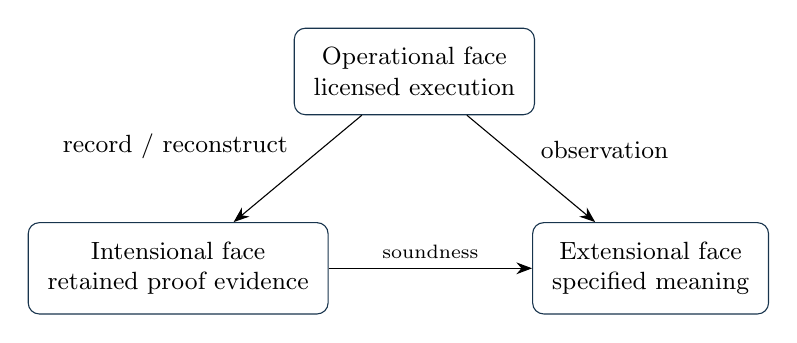
\begin{tikzpicture}[every node/.style={align=center,font=\small},
  >={Stealth[length=2mm]}]
\node[draw=ink,rounded corners,inner sep=7pt] (op) at (0,2.5)
  {Operational face\\licensed execution};
\node[draw=ink,rounded corners,inner sep=7pt] (proof) at (-3,0)
  {Intensional face\\retained proof evidence};
\node[draw=ink,rounded corners,inner sep=7pt] (meaning) at (3,0)
  {Extensional face\\specified meaning};
\draw[->] (op) -- node[above left] {record / reconstruct} (proof);
\draw[->] (proof) -- node[above,font=\scriptsize] {soundness} (meaning);
\draw[->] (op) -- node[above right] {observation} (meaning);
\end{tikzpicture}
\end{center}

For HOL, one extensional judgment is a \emph{semantic sequent}
$\Gamma\models_M A$: every admissible assignment in model $M$ satisfying the
assumptions in $\Gamma$ satisfies $A$. A Henkin model specifies the domains of
quantification, including which function values are available. Soundness
connects proof rules to this satisfaction relation; it does not identify the
model with the proof's syntax. Different proofs and execution orders can have
one semantic sequent. The arrows in the diagram require their stated
contracts and generally cannot be inverted.

\section{Rule signatures and the free cartesian multicategory}\label{sec:free}

\begin{definition}[Cartesian multicategory]
A cartesian multicategory over a type of sorts $\Sigma$ assigns to each finite
context $\Gamma : \mathrm{Fin}\,n \to \Sigma$ and sort $b$ a type
$\mathrm{Hom}(\Gamma; b)$, with variables $\mathrm{var}_i : \mathrm{Hom}(\Gamma;\Gamma_i)$
and simultaneous substitution
$\subst : \mathrm{Hom}(\Gamma;b) \times \prod_i \mathrm{Hom}(\Delta;\Gamma_i) \to \mathrm{Hom}(\Delta;b)$,
satisfying $\mathrm{var}_i[\sigma] = \sigma_i$, $t[\mathrm{var}] = t$ and
$t[\sigma][\tau] = t[\sigma[\tau]]$. A multifunctor over a map of sorts
$f : \Sigma \to \Sigma'$ sends $\mathrm{Hom}(\Gamma;b)$ to
$\mathrm{Hom}(f\circ\Gamma; f b)$, preserving variables and substitution.
\end{definition}
\lean{CartesianMulticategory, CartesianMulticategory.Functor}

Reindexing contexts by composition makes multifunctors compose without
transport; the list-indexed \name{MultiSortedClone} is the restriction to
contexts of the form $\ell.\mathrm{get}$. This is the many-sorted abstract clone
presentation; for the correspondence between clones, cartesian multicategories
and their internal languages see Saville, \emph{Clones, closed categories, and
combinatory logic}\cite{Saville}, which also recalls the multicategories introduced by Lambek
in \emph{Deductive systems and categories II}\cite{Lambek}. Lambek and Scott,
\emph{Introduction to Higher Order Categorical Logic}, treat the unary
deductive systems from which this generalizes.

\begin{proposition}[Multifunctors form a category]
Identity and composition of multifunctors satisfy the unit and associativity
laws. A multifunctor carries closed multimorphisms to closed multimorphisms.
\end{proposition}
\lean{CartesianMulticategory.Functor.id_comp, comp_id, comp_assoc, Functor.inhabited}

\begin{definition}[Rule signature, open derivations]
A rule signature $S$ assigns to each premise list $p_1\cdots p_k$ and conclusion
$c$ a type $S(p;c)$ of rule instances. Open derivations $\Term_S(\Gamma;b)$ are
generated by premise holes $\mathrm{var}_i$ and nodes
$r(t_1,\dots,t_k)$ with $r \in S(p;c)$ and $t_j \in \Term_S(\Gamma;p_j)$.
Substitution plugs derivations into holes. The generator of $r$ is
$\mathrm{gen}(r) = r(\mathrm{var}_1,\dots,\mathrm{var}_k)$.
\end{definition}
\lean{RuleSignature, RuleSignature.Term, Term.subst, RuleSignature.free, RuleSignature.gen}

\begin{theorem}[Freeness]\label{thm:free}
Open derivations with substitution form a cartesian multicategory $\Free(S)$.
For every cartesian multicategory $M$ and map of sorts $f$, restriction to
generators is an equivalence between multifunctors $\Free(S) \to M$ over $f$
and interpretations
\[ \textstyle\prod_{p,c}\; S(p;c) \longrightarrow \mathrm{Hom}_M(f\circ p;\, f c). \]
\end{theorem}
\lean{RuleSignature.universal, RuleSignature.functor_eq_of_gen, RuleSignature.lift_gen, Term.lift_subst}

\begin{theorem}[Derivability]
A sort is derivable in $\Free(S)$, i.e.\ has a closed derivation, exactly when
it lies in the inductive closure of the rule predicate $\exists r \in S(p;c)$.
Every multifunctor between free multicategories preserves derivability.
\end{theorem}
\lean{RuleSignature.derivable_iff_derives, RuleSignature.Derivable.map}

\begin{proposition}[Structural rules]
Holes may be discarded or reused, so $\Free(S)$ is cartesian; two holes of the
same sort remain distinct derivations. Generators are planar (each premise used
once, in order), and every closed derivation is planar.
\end{proposition}
\lean{Term.duplicate_holes_distinct, Term.gen_linear, Term.closed_linear}

Here the holes are metalevel proof dependencies for the fixed rule signature.
This construction does not authorize copying an object-level linear resource
or a capability. Such constraints must already be present in the judgment,
the allowed instances or a resource-sensitive composition. Planarity of these
closed terms is not an equivalence of arbitrary linear, symmetric and
cartesian object logics.

\begin{theorem}[Schematic level: instance actions]
If a map of sorts carries every rule instance to an instance of the mapped
premises and conclusion, it induces a multifunctor $\Free(S) \to \Free(S)$, and
derivability is closed under the map. Actions compose coherently: if two
actions compose on sorts and on instances to a third, acting by the two in turn
agrees with acting by the third on every derivation, up to the identification of
sorts. In particular substitution of formulas for atoms acts on the
intuitionistic and classical Hilbert multicategories, coherently with
composition of substitutions, so Hilbert derivability is substitution closed as
a consequence of freeness.
\end{theorem}
\lean{RuleSignature.InstanceAction, RuleSignature.actFunctor, RuleSignature.Derivable.act, RuleSignature.act_comp_heq, Hilbert.substFunctor, Hilbert.substFunctor_comp_heq, Hilbert.source_subst}

\begin{remark}[Contexts, binders and side conditions]
Object-level contexts and binders are part of the sorts: a HOL Light theorem
carries its hypothesis set and its terms their binders, and side conditions
such as freshness for abstraction are part of the rule-instance predicate. They
change the generators, not the kind of structure (Section~\ref{sec:kernels}).
Rules with one conclusion give a multicategory; multi-product consuming steps
are treated in Section~\ref{sec:execution}.
\end{remark}

\section{Kernels as free multicategories}\label{sec:kernels}

A kernel with a decidable rule-instance interface
$(\mathrm{W}, \mathrm{isInstance})$ presents the signature whose rule instances
are accepted witnesses.

\begin{theorem}[Derivability]
Kernel derivability coincides with closed derivability in the free
multicategory on the kernel's accepted witnesses.
\end{theorem}
\lean{RuleWitness.signature, RuleWitness.derivable_iff_derives}

\begin{theorem}[Certificate trees are closed morphisms]
For every conclusion $b$, closed derivations of $b$ correspond bijectively to
certificate trees of the kernel that its tree checker accepts with conclusion
$b$. Erasure to trees is injective.
\end{theorem}
\lean{RuleWitness.closedEquiv, RuleWitness.toDerivation_injective}

\begin{theorem}[Graphs unfold]
Replaying a shared derivation graph with the unfolding step yields exactly the
judgments of ordinary replay, now with closed derivations. Every node of an
accepted graph denotes a closed morphism of its conclusion, and therefore an
accepted certificate tree.
\end{theorem}
\lean{RuleWitness.termStep, RuleWitness.unfold_judgments, RuleWitness.unfold_root, RuleWitness.unfold_tree}

\begin{theorem}[Graphs present exactly the closed morphisms]
Every closed derivation is the unfolding of the last node of some accepted
derivation graph. With the previous theorem, accepted graphs present exactly
the closed morphisms of the free multicategory: sharing is a property of the
representation, never of the morphism.
\end{theorem}
\lean{RuleWitness.presented, RuleWitness.presented_block, DerivationGraph.replayWith_relocate, DerivationGraph.replayWith_append}

\begin{theorem}[Authored calculi]
For every validated authored calculus, the existing open derivations with
ordered premise contexts are exactly the terms of the free multicategory on its
rule applications, and plugging derivation vectors is substitution. Every
interpretation of the rule applications in a cartesian multicategory extends
uniquely to open derivations, preserving substitution. Accepted raw open proofs
decode computably to typed open derivations.
\end{theorem}
\lean{CertificateGSLT.ruleSignature, OpenDerivation.termEquiv, OpenDerivation.toTerm_bind, interpret_bind, interpret_unique, decodeOpen}

\begin{corollary}
The classifying category of every authored calculus (VibeITP, projected
Metamath snapshots, HOL Light's first-order calculus) is the category of
contexts of a free cartesian multicategory, with products by concatenation.
\end{corollary}
\lean{ClassifyingContext.instCategory, ClassifyingContext.concatIsLimit, OpenDerivation.termEquiv}

\begin{center}\small
\begin{tabularx}{\linewidth}{>{\raggedright\arraybackslash}p{0.27\linewidth}>{\raggedright\arraybackslash}X>{\raggedright\arraybackslash}p{0.33\linewidth}}
\toprule
Kernel & Rule-instance interface & Free multicategory \\
\midrule
Intuitionistic / classical Hilbert & finite codes, profile-gated excluded middle & \name{RuleWitness.signature (interface p)} \\
Extended Hilbert & classical codes and admitted definitions & \name{RuleWitness.signature (interface hs)} \\
HOL Light & ten rules and policy axioms & \name{RuleWitness.signature (ruleWitness policy)} \\
LRAT, RUP fragment & input clauses and RUP instances & \name{RuleWitness.signature (interface F)} \\
Authored calculi & rule applications & \name{CertificateGSLT.ruleSignature} \\
Grounded circular truth & ten codes over signed specifications & \name{RuleWitness.signature (Checking.interface system)} \\
Guarded atom rules, presentations & original rule codes & \name{Presentation.ruleWitness} \\
\bottomrule
\end{tabularx}
\end{center}

\section{Translations as multifunctors}\label{sec:translations}

By Theorem~\ref{thm:free}, a translation is determined by the images of rule
instances; derivability is preserved automatically.

\begin{theorem}[Faithful renamings]
A sort-preserving renaming of rule instances that is injective induces an
injective multifunctor.
\end{theorem}
\lean{RuleSignature.rename, RuleSignature.lift_rename_injective}

\begin{theorem}[Intuitionistic into classical]
The inclusion of intuitionistic into classical Hilbert rule instances induces a
faithful multifunctor that preserves but does not reflect derivability:
excluded middle is classically derivable and not intuitionistically derivable.
\end{theorem}
\lean{Hilbert.inclusion, Hilbert.inclusion_faithful, Hilbert.inclusion_not_reflecting}

\begin{theorem}[Classical into extended]
For every list of definitions, the inclusion of classical into extended rule
instances induces a faithful multifunctor. For admitted fresh definitions it is
conservative on claims in the old vocabulary. It is not full: citing a
definition is a derivation in the image of no classical derivation.
\end{theorem}
\lean{Extension.inclusion, Extension.inclusion_faithful, Extension.inclusion_conservative, Extension.inclusion_not_full}

\begin{theorem}[HOL Light into its first-order calculus]
Each accepted HOL Light rule instance is translated by the node step on its
canonical premise context and decoded to a typed open derivation of its rendered
conclusion. This determines a unique multifunctor from HOL Light's free rule
multicategory to the free multicategory of its first-order calculus over the
rendering of theorems. It preserves derivability, and for admitted axiom lists
reflects it: the calculus derives the rendering of a sequent exactly when HOL
Light derives a theorem with that sequent. Positive control: $\vdash p = p$ by
\textsf{REFL}; negative control: $\vdash \mathsf{F}$.
\end{theorem}
\lean{HOLLight.FirstOrder.generatorImage, translation, translation_unique, translation_derivable, translation_reflects, Kernel.reflexivity_translated, Kernel.falsity_not_translated}

\begin{theorem}[Sharing commutes with translation]
For any interpretation of a kernel's rule instances in a free multicategory,
translate a shared derivation graph node by node: check each node against its
source premise sorts and instantiate its rule image with the translated
premises. From translated entries this computes exactly the multifunctor images
of the unfolded entries. Hence every accepted graph translates with one rule
image per node, and the value at each node is the multifunctor image of that
node's closed derivation. In particular this holds for HOL Light graphs and the
translation above.
\end{theorem}
\lean{RuleWitness.liftStep, RuleWitness.liftStep_liftEntry, RuleWitness.replay_liftStep, RuleWitness.shared_translation, HOLLight.FirstOrder.shared_translation}

\begin{remark}
The existing compilation of first-order calculi into MM0 (the system of
\emph{Metamath Zero: The Cartesian Theorem Prover}\cite{Carneiro}) and the existing proof-graph
translation with shared lemmas complete the chain to MM0 at the level of
certificates. That existing translation builds each lemma with the same node
step over the cumulative context. On all 25 nodes of the three real HOL Light
exports of Section~\ref{sec:headline}, each of its lemmas coincides with the raw
rule proof from which the multifunctor's rule image is decoded, after renaming
premise positions to the lemma's parents. This is an executed comparison; the
general equality is open (Section~\ref{sec:open}).
\end{remark}

\section{Costs: logical work, sharing and extension}\label{sec:costs}

\begin{theorem}[Additivity]
Rule nodes are additive under substitution, each hole occurrence charged once:
$\size(t[\sigma]) = \size(t) + \sum_{i \in \occ(t)} \size(\sigma_i)$.
\end{theorem}
\lean{Term.size_subst}

\begin{theorem}[Affine translations are linear on trees]
If every rule image uses each premise at most once and has at most $c$ rule
nodes, the induced multifunctor satisfies $\size(F t) \le c \cdot \size(t)$.
\end{theorem}
\lean{RuleSignature.lift_size_le}

\begin{theorem}[SHARE: a contraction-induced expansion gap]
Translate the chain calculus (one premise per step) into the duplication
calculus by an image citing its premise twice. The $k$-chain has $k+1$ nodes;
its translation is a tree with $2^{k+1}-1$ nodes; the duplication calculus has
an accepted shared graph with $k+1$ rows for the same conclusion. The
contracting image is not affine.
\end{theorem}
\lean{Contraction.contraction_gap, Contraction.image_not_affine, ProofSharingBounds.no_tree_sizeSimulation_dag}

\begin{remark}[EXTEND]
Extension by definitions changes the multicategory: the inclusion is faithful
and conservative but not full (Section~\ref{sec:translations}), and literal
expansion of an admitted doubling chain has $2^{k+1}-1$ formula nodes from
encoded size at most $5(k+1)(k+2)$ (\name{PropositionalExtension.literal_expansion_gap}).
Sharing never changes the multicategory: a graph and its unfolded tree are one
morphism. In the sense of Cook and Reckhow, \emph{The Relative Efficiency of
Propositional Proof Systems}, a translation with polynomial size and time bounds
is a p-simulation. The proved size separation rules out polynomial-size
translation from the shared duplication certificates to trees; the
straightforward tree-to-DAG representation comparison has no such size
obstruction. An executed compiler-time bound must be supplied separately.
Extended resolution's polynomial
simulation of DRAT (Kiesl, Rebola-Pardo and Heule, \emph{Extended Resolution
Simulates DRAT}) is the corresponding EXTEND phenomenon for SAT certificates.
\end{remark}

\begin{proposition}[Time accounts]
The p-simulation of HOL Light proof graphs by MM0 has a degree-ten certificate
bound and a degree-ten declared time account; the declared time is at least the
weight of the lemmas the translation writes. An operational simulation derives
its clock from a finite-stack machine execution, and such clocks are positive.
\end{proposition}
\lean{HOLLight.FirstOrder.graphTranslate_weight, graphTime_ge_weight, Kernel.mm0Simulation, OperationalPSimulation.toPSimulation, OperationalPSimulation.time_positive}
\status{The HOL Light to MM0 time account is declared, bounded below by output
weight; its finite-stack realization is open.}

\section{Atomic multi-pattern steps and schedules}\label{sec:execution}

A step keeps some occurrences, consumes others and produces atoms, when its rule
admits them; this is the shape of multi-headed CHR simpagation (Di Giusto,
Gabbrielli and Meo, \emph{On the expressive power of multiple heads in CHR}) and
of chemical-style rewriting (Berry and Boudol, \emph{The Chemical Abstract
Machine}).

\begin{theorem}[Local characterization of replay]
Sequential replay with any local step accepts exactly when the final cache
extends the initial one, has one value per node, every reference points
backward, and every node's step on its looked-up premises yields its value.
\end{theorem}
\lean{DerivationGraph.replayWith, DerivationGraph.replayWith_iff_local, DerivationGraph.replayWith_judgmentStep}

\begin{theorem}[Schedule independence]
For a step that ignores physical reference positions, reordering a graph by any
permutation that keeps premises before consumers, with references relocated,
accepts exactly when the original order does (for topological originals), and
moves each node's value to its new position. A reordering that places a premise
after its consumer is refused. The numbers of local steps and premise lookups
are invariant. In particular judgment replay and unfolding are schedule
independent.
\end{theorem}
\lean{DerivationGraph.replayWith_permute, replayWith_permute_reflect, replayWith_permute_iff, replayWith_permute_refused, permute_lookups, replay_permute, RuleWitness.unfold_permute}

\begin{theorem}[Monotone steps are derivations]
Without consumption, running single-product steps is replay of the
corresponding derivation graph, and every accepted trace denotes, at every step,
a closed morphism of the free multicategory on the step rules. A monotone step
with several products runs exactly as the sequence of its single-product
components.
\end{theorem}
\lean{MultiPremiseSteps.run_monotone, run_monotone_unfolds, run_split}

\begin{theorem}[Consumption]
In an accepted trace a consumed occurrence is never cited again; occurrences
may be kept twice but not consumed twice, nor kept and consumed together. Two
steps competing for one occurrence lead to different stores, neither of which
can fire the other. Two steps with independent footprints (neither consumes what
the other cites, and the second cites no product of the first) fire in either
order, with the same live atoms up to the order of their products. In the
formalized tree of single-wire cuts, a composite has one internal wire fewer
than generators. The split/join process has two steps and two internal wires,
so that compositional syntax cannot represent it while preserving those
counts. This rules out that syntax as a complete account; it does not rule out
encoding processes in categories or alternative polycategorical frameworks.
\end{theorem}
\lean{MultiPremiseSteps.consumed_not_cited, Controls.consumption_not_confluent, Controls.keep_twice, Controls.take_twice_refused, independent_commute, Controls.independent_steps_commute, PolyComposite.wires_add_one, process_not_polycategorical}

\begin{remark}[What the correspondence keeps]
Kept: rule witnesses, ordered and repeated premise occurrences, every
conclusion, acceptance including refusal of unused bad steps, and step counts.
Forgotten: the order of independent steps; sharing (a graph and its unfolding
are one morphism); the identity of steps not used by the selected root.
Consumption keeps resources linear and needs monoidal composition of
processes; negative reads are outside this step shape.
\end{remark}

\section{Admission and revalidation of retained evidence}\label{sec:revalidation}

\begin{theorem}[Exact revalidation]
For a graph accepted under one interface, rechecking each node's rule instance
against another interface, with premises read from the retained cache, succeeds
exactly when the mapped graph replays under the new interface to the same
cache. Admitted extensions (witness maps keeping accepted instances accepted)
transport evidence; checked judgments are reusable in larger rule systems; a
retained source-address schedule replays to the identical state under a new
interface accepting each instance it used.
\end{theorem}
\lean{DerivationGraph.revalidate_iff, replay_extend, CheckedJudgment.extend, BorrowedCursor.run_reinterpret}

\begin{theorem}[Propositional admission joined to retained evidence]
Every accepted intuitionistic graph is accepted classically with the same cache.
An accepted extended graph remains accepted when further admitted definitions are
appended. Classical evidence for excluded middle is refused on intuitionistic
revalidation; evidence citing a definition that was replaced by a different
admitted definition is refused.
\end{theorem}
\lean{Revalidation.intuitionistic_to_classical, Revalidation.checkDAG_append, Controls.em_refused_intuitionistically, Controls.worked_extended, Controls.worked_changed_refused}

\section{Module coverage and the LRAT action adapter}\label{sec:modules}

\begin{theorem}[HOL Light kernel module]
The first-order calculus of HOL Light over an axiom list renders as a portable
module that the verified reader and the original validator load exactly. The
loaded package derives the rendering of a sequent exactly when HOL Light derives
a theorem with that sequent, for admitted axiom lists.
\end{theorem}
\lean{HOLLight.FirstOrder.kernelModule, kernelModule_read, kernelModule_faithful}
\status{Exported for the bare kernel: 147 rules, 991\,249 bytes, read back through
the actual reader and validator.}

\begin{theorem}[LRAT actions]
A reverse-unit-propagation addition is a multi-premise rule instance whose
premises are its hinted clauses, and it is sound. An LRAT action stream compiles,
with identifiers resolved to positions and deletions enforced, to a derivation
graph; acceptance of that graph with an empty clause refutes the formula, and
every action denotes a closed morphism of the free multicategory on RUP
instances. A resolution-asymmetric addition need not be implied, so it is not a
rule instance of this calculus.
\end{theorem}
\lean{PropositionalLRATActions.rupCheck_sound, check_sound, check_graph, check_unfolds, rat_not_implied, rat_not_rule_instance}

\begin{center}\small
\begin{tabularx}{\linewidth}{>{\raggedright\arraybackslash}p{0.24\linewidth}>{\raggedright\arraybackslash}X>{\raggedright\arraybackslash}p{0.24\linewidth}}
\toprule
Native profile & Faithful presentation & Portable module \\
\midrule
VibeITP & authored calculus, \name{kernel_derives_iff_classifyingArrow} & yes, 123 schemas \\
Metamath snapshot & projected authored calculus & yes, 25 schemas \\
HOL Light kernel & first-order calculus, \name{kernelModule_faithful} & yes, 147 rules \\
Hilbert, extended Hilbert & exact rule codes; sorted Hilbert source presentation also exists & not qualified here \\
LRAT (RUP fragment) & action calculus, \name{check_sound} & no (RUP is a computed check) \\
Grounded circular truth & signed evidence rules, \name{judgment_coverage} & no (base admission is a parameter) \\
MM0, Megalodon & owned by the active MM0 lane & not covered here \\
Rho, MeTTa equations, GSLT recipes & retained workers (\emph{Abstract Machines}, Section~13) & open \\
\bottomrule
\end{tabularx}
\end{center}

\section{The costed HOL Light to MM0 translation}\label{sec:headline}

The existing receiver replays real HOL Light exports, lowers the registered
receipts to proof graphs, translates each node through its first-order step,
compiles the shared lemmas to MM0 saved proofs, checks them in Lean and prints
specification and proof texts. The reference MM0 tools then compile the proof
text and verify the binary against the specification.

\begin{center}\small
\begin{tabular}{@{}lrrrrrrr@{}}
\toprule
Export & events & spec & MMU & emit & MMB & compile & verify \\
 & & (MB) & (MB) & (s) & (bytes) & (s) & (s) \\
\midrule
\textsf{T\_DEF} & 1 & 26.2 & 40.1 & 14.4 & 220\,512 & 0.58 & 0.13 \\
\textsf{TRUTH} & 8 & 22.6 & 252.2 & 2166 & 223\,536 & 4.08 & 0.14 \\
\bottomrule
\end{tabular}
\end{center}

Emission includes the Lean-side check and printing of each text: for
\textsf{TRUTH}, lowering, node translation and shared-proof compilation take
under a minute, while checking and printing the proof text and the MM1 text take
16 and 19 minutes at a peak of 2.8\,GiB. The specification encodes the fixed
147-rule presentation and dominates the binary certificate; the eight-node
proof adds about three kilobytes to it. The
proved bounds are polynomial of degree ten with generous constants; the measured
growth is far below them. The text formats and the in-process checking dominate
wall-clock cost, not the reference verifier. These are executed times of the
existing binary and are kept separate from the logical work and the declared
time account of Section~\ref{sec:costs}, which the following table reports in
the measures of the proved bounds (graph size $N$, lemma-certificate weight,
first-order rule nodes and declared time).

\begin{center}\small
\begin{tabular}{@{}lrrrrr@{}}
\toprule
Export & nodes & $N$ & certificate weight & rule nodes & declared time \\
\midrule
\textsf{T\_DEF} & 1 & 371\,826 & 185\,913 & 1 & $1.9\times10^{22}$ \\
\textsf{TRUTH} & 8 & 3\,610\,421 & 4\,562\,433 & 1\,505 & $1.3\times10^{24}$ \\
core \textsf{bool} & 16 & 43\,070\,295 & 24\,292\,374 & 1\,513 & $5.2\times10^{28}$ \\
\bottomrule
\end{tabular}
\end{center}

These measurements are historical qualification runs of the receiver frozen
on 13 October 2026. They have not been reproduced with a rebuilt receiver in
the present source state and are not current performance guarantees.

The certificate weight is $1.26\,N$ on \textsf{TRUTH}, while the proved bound
$(35\cdot10^{12}+2)(N+1)^{10}$ exceeds $10^{78}$: the degree-ten bound is
sound and very loose. The declared time is dominated by its fourth-power
comparison term and says nothing about executed time. On the sixteen-event core
\textsf{bool} export, the executed compilation to MM0 saved proofs exhausted
its available memory at the last of its sixteen nodes, after assembling a
156-rule presentation; memory, not time, bounds the executed translation there.

\section{Status ledger}\label{sec:ledger}

Entries marked ``proved'' are checked without \code{sorry}, custom axioms or
native decision. Entries marked ``open'' are obligations, not proved claims.
Axioms are those reported by \code{#print axioms} on the listed declaration:
\textsf{P} = \code{propext}, \textsf{C} = \code{Classical.choice},
\textsf{Q} = \code{Quot.sound}; ``none'' means no axioms.

% Generated from the axiom audit; do not edit by hand.
\begin{small}
\begin{longtable}{@{}l>{\raggedright\arraybackslash}p{0.37\linewidth}>{\raggedright\arraybackslash}p{0.34\linewidth}ll@{}}
\toprule
Part & Claim & Lean declaration & Axioms & Status\\
\midrule
\endhead
A1 & Freeness: multifunctors out of open derivations are interpretations of rule instances & \name{RuleSignature.universal} & Q & proved\\
A1 & A multifunctor is determined by its generators & \name{RuleSignature.functor_eq_of_gen} & Q & proved\\
A1 & Extension agrees with the interpretation on generators & \name{RuleSignature.lift_gen} & none & proved\\
A1 & Extension preserves substitution & \name{RuleSignature.Term.lift_subst} & Q & proved\\
A1 & Right unit law & \name{RuleSignature.Term.subst_vars} & Q & proved\\
A1 & Associativity of substitution & \name{RuleSignature.Term.subst_subst} & Q & proved\\
A1 & Closed derivability is the inductive rule closure & \name{RuleSignature.derivable_iff_derives} & PQ & proved\\
A1 & Closed derivations are planar & \name{RuleSignature.Term.closed_linear} & P & proved\\
A1 & Generators are planar & \name{RuleSignature.Term.gen_linear} & PQ & proved\\
A1 & Holes of equal sort stay distinct & \name{RuleSignature.Term.duplicate_holes_distinct} & P & proved\\
A1 & Stable instance actions induce multifunctors & \name{RuleSignature.actFunctor} & PQ & proved\\
A1 & Derivability is closed under instance actions & \name{RuleSignature.Derivable.act} & PQ & proved\\
A1 & Substitution acts on Hilbert multicategories & \name{Hilbert.substFunctor} & PQ & proved\\
A1 & Hilbert derivability is substitution closed & \name{Hilbert.source_subst} & PQ & proved\\
A1 & Instance actions compose coherently & \name{RuleSignature.act_comp_heq} & PQ & proved\\
A1 & Substitution multifunctors compose coherently & \name{Hilbert.substFunctor_comp_heq} & PCQ & proved\\
A1 & Multifunctors compose associatively & \name{CartesianMulticategory.Functor.comp_assoc} & Q & proved\\
A1 & Multifunctors preserve closed morphisms & \name{CartesianMulticategory.Functor.inhabited} & none & proved\\
A1 & Kernel derivability is closed derivability & \name{RuleWitness.derivable_iff_derives} & PQ & proved\\
A1 & Closed morphisms are accepted certificate trees & \name{RuleWitness.closedEquiv} & PQ & proved\\
A1 & Erasure to trees is injective & \name{RuleWitness.toDerivation_injective} & PQ & proved\\
A1 & Unfolding replay agrees with judgment replay & \name{RuleWitness.unfold_judgments} & PQ & proved\\
A1 & Every accepted graph node unfolds to a closed morphism & \name{RuleWitness.unfold_root} & PQ & proved\\
A1 & Every accepted graph node yields an accepted tree & \name{RuleWitness.unfold_tree} & PQ & proved\\
A1 & Every closed morphism is the unfolding of an accepted graph root & \name{RuleWitness.presented} & PCQ & proved\\
A1 & Presented blocks combine into one graph & \name{RuleWitness.presented_block} & PCQ & proved\\
A1 & Authored open derivations are free-multicategory terms & \name{CertificateGSLT.OpenDerivation.termEquiv} & PQ & proved\\
A1 & Plugging is substitution & \name{CertificateGSLT.OpenDerivation.toTerm_bind} & PQ & proved\\
A1 & Interpretation of open derivations preserves substitution & \name{CertificateGSLT.interpret_bind} & PQ & proved\\
A1 & Interpretation of open derivations is unique & \name{CertificateGSLT.interpret_unique} & PQ & proved\\
A1 & Computable decoding of accepted raw open proofs & \name{CertificateGSLT.decodeOpen} & PCQ & proved\\
A2 & Translations preserve derivability & \name{RuleSignature.Derivable.map} & Q & proved\\
A2 & Injective renamings induce faithful multifunctors & \name{RuleSignature.lift_rename_injective} & Q & proved\\
A2 & Intuitionistic into classical: faithful & \name{Hilbert.inclusion_faithful} & PQ & proved\\
A2 & Intuitionistic into classical: not reflecting & \name{Hilbert.inclusion_not_reflecting} & PCQ & proved\\
A2 & Classical into extended: faithful & \name{Extension.inclusion_faithful} & PQ & proved\\
A2 & Classical into extended: conservative & \name{Extension.inclusion_conservative} & PCQ & proved\\
A2 & Classical into extended: not full & \name{Extension.inclusion_not_full} & PCQ & proved\\
A2 & HOL Light into its first-order calculus: multifunctor & \name{HOLLight.FirstOrder.translation} & PCQ & proved\\
A2 & That multifunctor is determined by rule images & \name{HOLLight.FirstOrder.translation_unique} & PCQ & proved\\
A2 & It preserves derivability & \name{HOLLight.FirstOrder.translation_derivable} & PCQ & proved\\
A2 & It reflects derivability & \name{HOLLight.FirstOrder.translation_reflects} & PCQ & proved\\
A2 & Positive control: REFL translated & \name{HOLLight.FirstOrder.Kernel.reflexivity_translated} & PCQ & proved\\
A2 & Negative control: F not derivable & \name{HOLLight.FirstOrder.Kernel.falsity_not_translated} & PCQ & proved\\
A2 & Node-by-node translation of one node is the multifunctor image & \name{RuleWitness.liftStep_liftEntry} & PCQ & proved\\
A2 & Shared translation commutes with unfolding & \name{RuleWitness.replay_liftStep} & PCQ & proved\\
A2 & Accepted graphs translate with sharing, coherently & \name{RuleWitness.shared_translation} & PCQ & proved\\
A2 & HOL Light graphs translate with sharing, coherently & \name{HOLLight.FirstOrder.shared_translation} & PCQ & proved\\
A3 & Logical work is additive under substitution & \name{RuleSignature.Term.size_subst} & PQ & proved\\
A3 & Affine translations are linear on trees & \name{RuleSignature.lift_size_le} & PCQ & proved\\
A3 & Contraction: linear source, exponential tree, linear graph & \name{Contraction.contraction_gap} & PCQ & proved\\
A3 & The contracting image is not affine & \name{Contraction.image_not_affine} & PQ & proved\\
A3 & Trees do not size-simulate graphs (existing) & \name{ProofSharingBounds.no_tree_sizeSimulation_dag} & PCQ & proved\\
A3 & Literal expansion of definitions is exponential (existing) & \name{PropositionalExtension.literal_expansion_gap} & PCQ & proved\\
A3 & HOL graph to MM0 certificate bound, degree 10 (existing) & \name{HOLLight.FirstOrder.graphTranslate_weight} & PCQ & proved\\
A3 & Declared time is at least the written lemma weight & \name{HOLLight.FirstOrder.graphTime_ge_weight} & PCQ & proved\\
A3 & MM0 p-simulates HOL Light graphs, declared time (existing) & \name{HOLLight.FirstOrder.Kernel.mm0Simulation} & PCQ & proved\\
A3 & Operational clocks are positive (existing) & \name{ProofSystems.OperationalPSimulation.time_positive} & PCQ & proved\\
A4 & Sequential replay is local & \name{DerivationGraph.replayWith_iff_local} & PCQ & proved\\
A4 & Schedule independence (forward) & \name{DerivationGraph.replayWith_permute} & PCQ & proved\\
A4 & Schedule independence (reflection) & \name{DerivationGraph.replayWith_permute_reflect} & PCQ & proved\\
A4 & Schedule independence (both directions) & \name{DerivationGraph.replayWith_permute_iff} & PCQ & proved\\
A4 & Dependency-violating schedules are refused & \name{DerivationGraph.replayWith_permute_refused} & PCQ & proved\\
A4 & Lookup count is schedule invariant & \name{DerivationGraph.permute_lookups} & PCQ & proved\\
A4 & Replayed blocks relocate into larger caches & \name{DerivationGraph.replayWith_relocate} & PCQ & proved\\
A4 & Unfoldings are schedule invariant & \name{RuleWitness.unfold_permute} & PCQ & proved\\
A4 & Monotone single-product steps are graph replay & \name{MultiPremiseSteps.run_monotone} & PQ & proved\\
A4 & Monotone traces denote closed morphisms & \name{MultiPremiseSteps.run_monotone_unfolds} & PQ & proved\\
A4 & Monotone multi-product steps split & \name{MultiPremiseSteps.run_split} & PQ & proved\\
A4 & Consumption is linear & \name{MultiPremiseSteps.consumed_not_cited} & PQ & proved\\
A4 & Consumption is not confluent & \name{MultiPremiseSteps.Controls.consumption_not_confluent} & PQ & proved\\
A4 & Independent consuming steps commute up to product order & \name{MultiPremiseSteps.independent_commute} & PQ & proved\\
A4 & Control: two independent consuming steps commute & \name{MultiPremiseSteps.Controls.independent_steps_commute} & PQ & proved\\
A4 & Split/join exceeds tree-shaped single-wire-cut composition & \name{MultiPremiseSteps.process_not_polycategorical} & PQ & proved\\
C & HOL Light kernel module loads exactly & \name{HOLLight.FirstOrder.kernelModule_read} & PCQ & proved\\
C & Loaded HOL Light module is faithful & \name{HOLLight.FirstOrder.kernelModule_faithful} & PCQ & proved\\
C & VibeITP module loads exactly (existing) & \name{VibeITP.CheckingMachine.kernelModule_read} & PCQ & proved\\
C & RUP instances are sound & \name{PropositionalLRATActions.rupCheck_sound} & PQ & proved\\
C & LRAT action checker is sound & \name{PropositionalLRATActions.check_sound} & PQ & proved\\
C & LRAT actions denote closed morphisms & \name{PropositionalLRATActions.check_unfolds} & PQ & proved\\
C & RAT additions are not RUP rule instances & \name{PropositionalLRATActions.rat_not_rule_instance} & PQ & proved\\
C & Positive control: RUP refutation & \name{PropositionalLRATActions.Controls.xor_accepted} & PQ & proved\\
C & Negative control: deleted premise & \name{PropositionalLRATActions.Controls.deleted_premise_refused} & PQ & proved\\
C & RAT proof classified as extension & \name{PropositionalLRATActions.Controls.rat_refused} & PQ & proved\\
D & Revalidation is exact & \name{DerivationGraph.revalidate_iff} & PCQ & proved\\
D & Admitted extensions transport evidence & \name{DerivationGraph.replay_extend} & PCQ & proved\\
D & Checked judgments extend to larger rule systems & \name{DerivationGraph.CheckedJudgment.extend} & none & proved\\
D & Retained schedules reinterpret under accepting interfaces & \name{DerivationGraph.BorrowedCursor.run_reinterpret} & PQ & proved\\
D & Intuitionistic evidence is classical evidence & \name{Revalidation.intuitionistic_to_classical} & PCQ & proved\\
D & Evidence survives appended admitted definitions & \name{Revalidation.checkDAG_append} & PCQ & proved\\
D & Negative control: excluded middle refused & \name{Revalidation.Controls.em_refused_intuitionistically} & P & proved\\
D & Positive control: extended definitions & \name{Revalidation.Controls.worked_extended} & PCQ & proved\\
D & Negative control: changed definition & \name{Revalidation.Controls.worked_changed_refused} & PQ & proved\\
G & Ten source evidence rules have an exact executable interface & \name{KripkeTruth.Checking.interface} & P & proved\\
G & Accepted certificates yield original source evidence & \name{KripkeTruth.Checking.check_sound} & PQ & proved\\
G & Certificate coverage is exactly source evidence & \name{KripkeTruth.Checking.coverage} & PCQ & proved\\
G & Certificates characterize least-fixed-point membership & \name{KripkeTruth.Checking.judgment_coverage} & PCQ & proved\\
G & Closed categorical proofs characterize grounded judgments & \name{KripkeTruth.Checking.closed_proof_iff_grounded} & PQ & proved\\
G & Finite decision and certificate authority coincide & \name{KripkeTruth.Checking.finite_decision_iff_certificate} & PCQ & proved\\
G & Completed unknown excludes both certificate polarities & \name{KripkeTruth.Checking.finite_undetermined_iff_no_certificates} & PCQ & proved\\
G & Positive control: admitted fact & \name{KripkeTruth.Checking.Controls.fact_accepts} & P & proved\\
G & Negative control: forged negative conclusion & \name{KripkeTruth.Checking.Controls.forged_false_refuses} & P & proved\\
G & Negative control: unsupported truth reference & \name{KripkeTruth.Checking.Controls.absent_premise_refuses} & P & proved\\
G & Liar has no certificate at either polarity & \name{KripkeTruth.Checking.Controls.liar_has_no_certificate} & PCQ & proved\\
G & Negative control: unadmitted negative base leaf & \name{KripkeTruth.Checking.Controls.false_base_leaf_refuses} & P & proved\\
G & Negative control: cyclic proof-graph reference & \name{KripkeTruth.Checking.Controls.cyclic_graph_refuses} & P & proved\\
E & Weighted state and branch-cost sequencing is associative & \name{LayerEffects.Spec.bind_assoc} & PCQ & proved\\
E & A write and a read need not commute & \name{LayerEffects.Controls.put_get_not_comm} & PCQ & proved\\
E & The specified distribution-over-finite-sets law is impossible & \name{NondeterminismProbability.no_distributiveLaw} & PCQ & proved\\
E & Surviving answers cannot recover every failed-branch charge & \name{LayerEffects.Spec.no_failed_cost_recovery} & PCQ & proved\\
E & Marginals cannot determine same-world conjunction & \name{EvidenceSpaces.no_same_world_conjunction_from_marginals} & PQ & proved\\
\midrule
A3 & Finite-stack realization of the HOL Light to MM0 translation & --- & --- & open\\
A2 & Existing shared-lemma HOL translation equals the node-by-node translation & --- & --- & open\\
A4 & Free symmetric monoidal category of consuming processes & --- & --- & open\\
C & Portable modules for rho, MeTTa equations, recipes, rule-code kernels & --- & --- & open\\
\bottomrule
\end{longtable}
\end{small}


\section{Open problems}\label{sec:open}

\begin{enumerate}
\item \textbf{Finite-stack realization of the HOL Light to MM0 translation.} The
  certificate bound is proved and the declared time account is bounded below by
  output weight, but no finite-stack machine computing the translation is
  given; a pushdown transducer for planar rule images is the natural first case.
\item \textbf{The existing lemma translation.} The generic node-by-node
  translation commutes with unfolding; prove that the existing shared-lemma HOL
  Light translation, which works over cumulative contexts and raw proofs,
  computes the same per-node rule images.
\item \textbf{Monoidal processes for consuming steps.} Independent consuming steps
  commute and the split/join example exceeds tree-shaped single-wire cuts; the free
  symmetric monoidal category of processes, with traces identified exactly up to
  independence, is not formalized.
\item \textbf{Memory of the executed MM0 compilation.} On a sixteen-event export
  with ten definitional roots, the existing compiler exhausted its memory allowance
  while compiling the last of sixteen shared proofs; witness sharing in the
  compiled MM0 proofs is the evident target.
\item \textbf{Remaining portable modules.} Rho, MeTTa equation and authored
  recipe kernels, and the propositional rule-code kernels, have faithful checkers
  but no portable module presentation.
\end{enumerate}

\begin{thebibliography}{9}
\bibitem{Nyayabindu}
Dharmakirti. \emph{Nyayabindu}, chapters I--III, with Dharmottara's commentary.
English translation in Th. Stcherbatsky, \emph{Buddhist Logic}, vol.~II,
Bibliotheca Buddhica XXVI, 1930.

\bibitem{ChalmersJackson}
D.~J. Chalmers and F. Jackson. Conceptual analysis and reductive explanation.
\emph{The Philosophical Review} 110 (2001), 315--361, Section~2.
\url{https://consc.net/papers/analysis.html}.

\bibitem{ChalmersWorld}
D.~J. Chalmers. \emph{Constructing the World}. Oxford University Press, 2012,
especially chapters 1--3 and the sixth excursus on totality and indexical truths.
\url{https://consc.net/constructing-the-world/}.

\bibitem{KripkeTruth}
S.~A. Kripke. Outline of a theory of truth.
\emph{The Journal of Philosophy} 72 (1975), 690--716.

\bibitem{Lambek}
J. Lambek. Deductive systems and categories II: standard constructions and
closed categories. In \emph{Category Theory, Homology Theory and their
Applications I}, Lecture Notes in Mathematics 86, Springer, 1969, 76--122.

\bibitem{Saville}
P. Saville. Clones, closed categories, and combinatory logic.
\emph{FoSSaCS 2024}, Lecture Notes in Computer Science 14575, pp.~160--181.
\url{https://arxiv.org/abs/2405.01675}.

\bibitem{Carneiro}
M. Carneiro. Metamath Zero: the Cartesian theorem prover.
Preprint, 2019. \url{https://arxiv.org/abs/1910.10703}.

\bibitem{McTT}
J. Jang, A. Gaulin, J.~Z.~S. Hu and B. Pientka.
McTT: A verified kernel for a proof assistant.
\emph{Proceedings of the ACM on Programming Languages}, ICFP, 2025.
\url{https://doi.org/10.1145/3747511}.

\bibitem{TTobs}
L. Pujet and N. Tabareau. Observational equality: now for good.
\emph{Proceedings of the ACM on Programming Languages} 6, POPL, 2022.
\url{https://doi.org/10.1145/3498693}.
\end{thebibliography}

\end{document}
